\section{\AP{}Key Lemma: Maximal Under Approximations are Semantically Finite}
\label{sec:proof-key-lemma}

\AP We can now start to describe the constructions used to prove the "Key Lemma"~\ref{lemma:bound_size_refinements}. Given a fixed "C2RPQ" $\gamma$ and a fixed $k \geq 1$,
we call a ""trio"" any triple $(\alpha,\rho,\fun)$ such that 
$\alpha \in \Tw$,
$\rho \in \Refin(\gamma)$ and 
$\fun$ is a "strong onto homomorphism" from $\rho$ to $\alpha$. 
For clarity, we will denote such a "trio" by simply ``$\fun\colon \rho \surj \alpha$''. 
Using this terminology, in order to prove \Cref{lemma:bound_size_refinements}, it is sufficient (and necessary) to show that:
\begin{center}
	for every "trio" $\fun\colon \rho \surj \alpha$,
	there exists another "trio" $\fun'\colon \rho' \surj \alpha'$\\
	"st" $\alpha \contained \alpha'$ and $\rho'\in \Refin[\leq \l](\gamma)$.
\end{center}

\begin{remark}
	\AP\label{rk:key-lemma-tw1}
	Note that this section does not use the fact that $k \geq 2$. In particular,
	\Cref{lemma:bound_size_refinements} holds for $k=1$. However,
	\Cref{coro:equivalence_under_approx_homomorphism_twk} does not apply,
	and $\MUA{\gamma}{\Tw[1]}$ (which we are interested in)
	is not equivalent to $\MUAHom{\gamma}{\Tw[1]}$ (which is shown to be computable by \Cref{lemma:bound_size_refinements}). We discuss this case in further details in \Cref{sec:acyclic-queries}.
\end{remark}

\subsection{\AP{}Local Acyclicity}
Our first construction, which will ultimately allow us to bound the size of "atom refinements",
shows that we can assume "wlog" that they "induce" "acyclic paths" in a "fine tagged 
tree decomposition" of $\fun$.

\begin{lemma}
    \AP\label{lemma:locally_acyclic_treedec}
    For any "trio" $\fun\colon \rho \surj \alpha$, there exists a "trio" $\fun'\colon \rho' \surj \alpha'$ and a "fine tagged tree decomposition" $(T', \bagmap', \tagmap')$ of "width" at most 
    $k$ of $\fun'$ such that
    $\alpha \contained \alpha'$, $\nbatoms{\rho'} \leq \nbatoms{\rho}$ and every "atom refinement" of
    $\rho'$ "induces" an "acyclic path" in the tree $T'$, in which case
    we say that $(T', \bagmap', \tagmap')$ is ""locally acyclic""
	"wrt" $f'$.
\end{lemma}

% \begin{figure}
%     \centering%
%     \includegraphics[width=.5\linewidth]{acyclic-induced-path1.pdf}%
%     \includegraphics[width=.5\linewidth]{acyclic-induced-path2.pdf}
%     \caption{%
%         \AP\label{fig:path-induced}%
%         Changing an "atom refinement" of $\gamma$ so that it induces an "acyclic path" in $T$.
%         \textcolor{red}{Attention: use "contraction"}
%     }
% \end{figure}
\begin{figure*}[tbp]
	\centering
	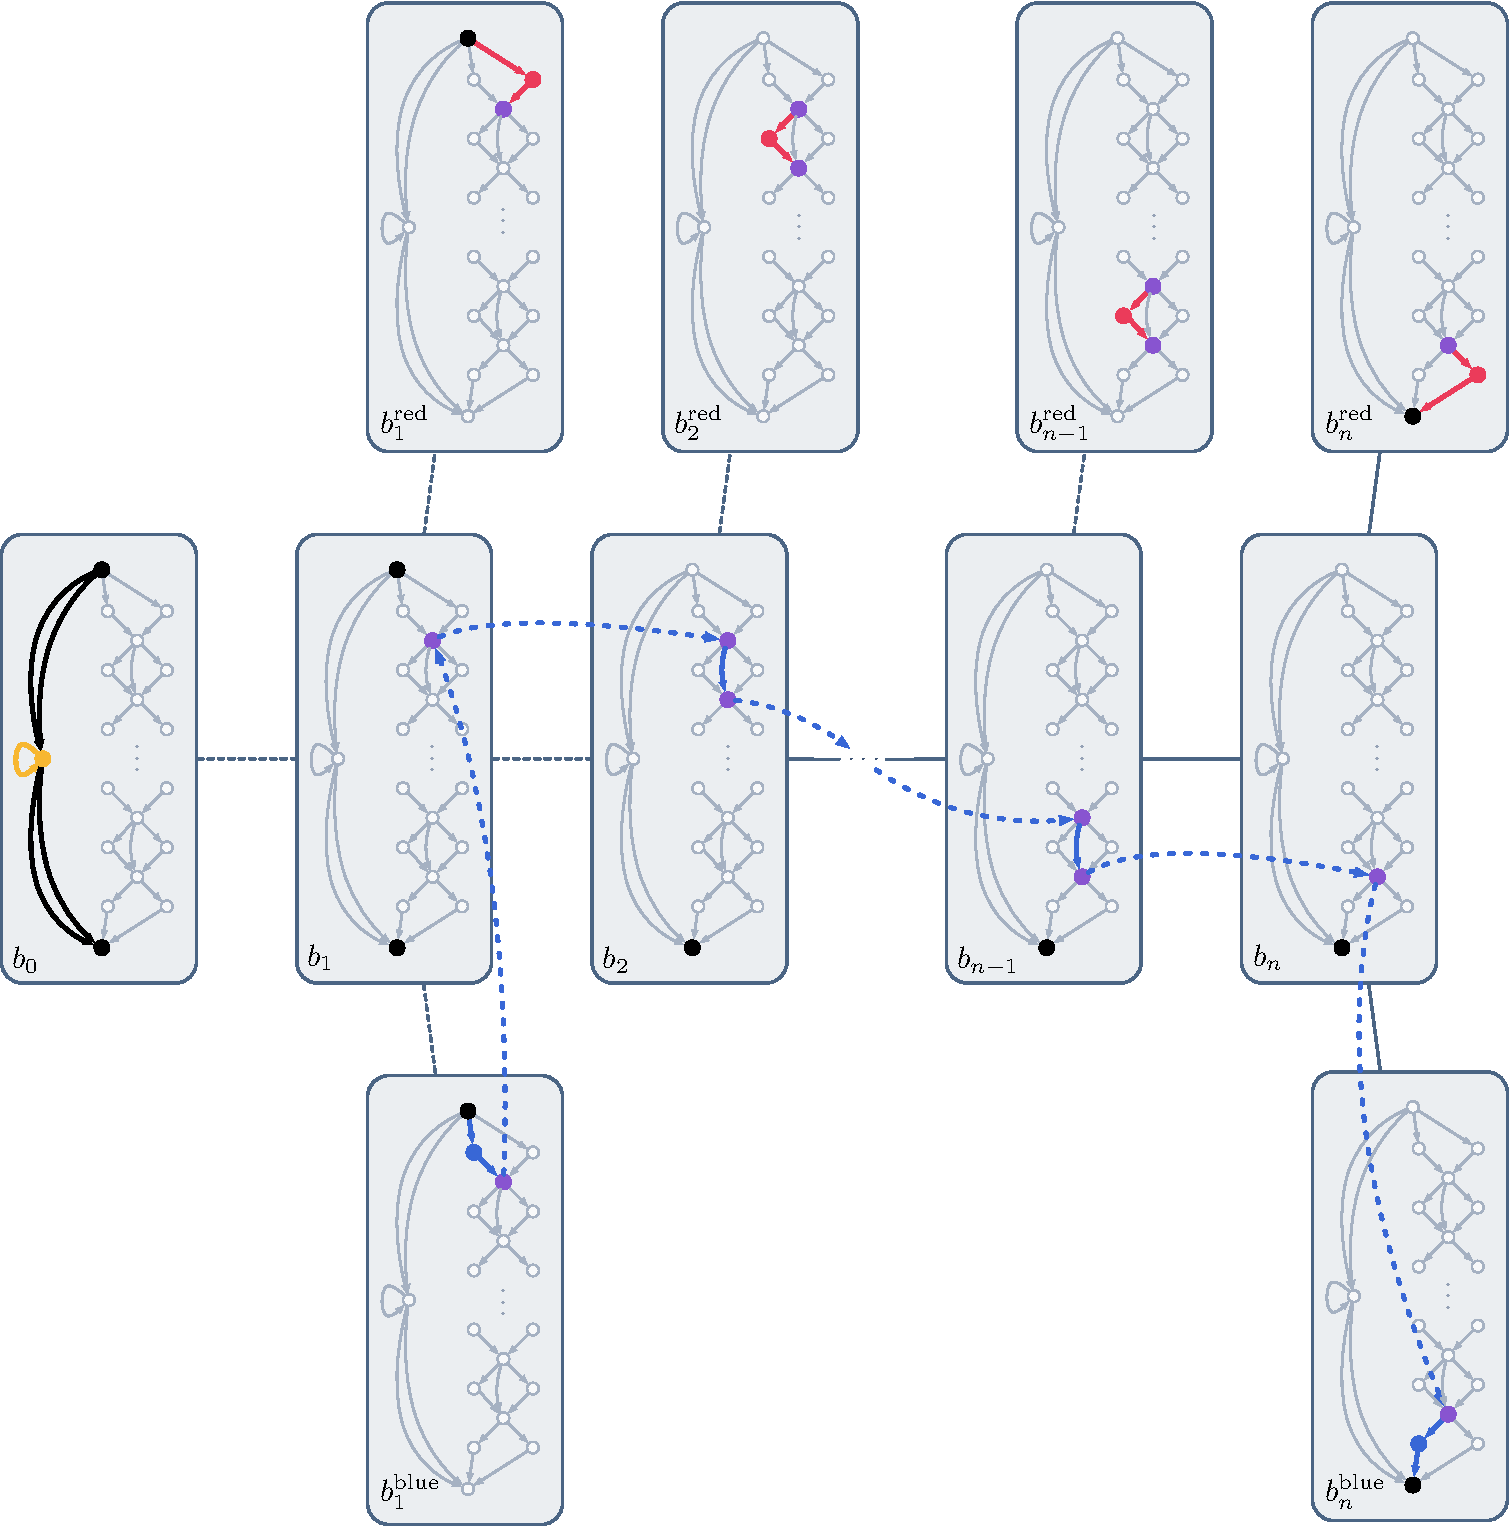
\includegraphics[width=\linewidth]{trio-tree-dec-acyclic.pdf}
	\caption{
		\AP\label{fig:path-induced}
        Changing the blue "atom refinement" of $\gamma$ (see \Cref{fig:trio-tree-dec})
		so that it induces an "acyclic path".
	}
\end{figure*}

Note that the fact that $f'$ is a "trio" implies in particular that
$\rho'$ is a "refinement" of $\gamma$.
The construction behind \Cref{lemma:locally_acyclic_treedec} is
illustrated in \Cref{fig:path-induced}.
\begin{notation}
	\AP\label{nota:nice-tree-dec}
	When two "bags" are linked by a dashed
	edge (as in \Cref{fig:trio-tree-dec,fig:path-induced}), it means
	that there is another "bag" in between them, which is there
	to ensure the fact that the "decomposition@tree decomposition" is "fine".
	The vertices contained in this extra bag are exactly the intersection of
	the vertices contained by its two neighbours, and no atom is tagged inside.
\end{notation}

\begin{proof}[Informal proof of \Cref{lemma:locally_acyclic_treedec}]
    Start with a "trio"
    $\fun\colon \rho \surj \alpha$, and let $(T, \bagmap, \tagmap)$ be a "fine tagged tree decomposition" of
    $\fun$. Consider an "atom refinement"
    $\pi \defeq z_0 \atom{L_1} z_1 \atom{L_2} \cdots \atom{L_n} z_n$
    in $\rho$ of some atom $x \atom{L} y$ (with $z_0 \defeq x$ and $z_n \defeq y$),
    and assume that it "induces"
    a "cyclic path" in $T$--- see "eg" \Cref{fig:trio-tree-dec}. It means that some variables $z_i$ and $z_j$ are mapped by $\fun$
    to the same bag of $T$, somewhere along the path "induced" by $\pi$. It suffices then to "condense" $\rho$
    by replacing the "atoms" $z_i \atom{L_{i+1}} \cdots \atom{L_j} z_j$ by a single
    "atom" $z_i \atom{\contract{L_{i+1} \cdots L_j}} z_j$.
    We thus obtain a new "refinement" $\rho'$ of $\gamma$.
    Then define $\alpha'$ be simply adding an atom $\fun(z_i) \atom{L_{i+1} \cdots L_j} \fun(z_j)$.
    The definitions of $\fun'$ and $(T',\bagmap',\tagmap')$ are then straightforward---potentially,
    $\alpha'$ should be restricted to the image of $\fun'\colon \rho' \homto \alpha'$ so that $\fun'$ is still "strong onto" by using \Cref{fact:restriction_tagged_treedec}. Crucially, $\alpha \contained \alpha'$, and $\alpha'$ still has "tree-width" at most $k$ 
    since we picked $\fun(z_i)$ and $\fun(z_j)$ so that they belonged to the same bag of $T$: therefore, adding an "atom" between them is innocuous.
	We then iterate this construction for every "atom refinement".
\end{proof}

\Cref{fig:path-induced} shows the "fine tagged tree decomposition" $(T',\bagmap',\tagmap')$
obtained by applying the previous construction to the "decomposition@fine tagged tree decomposition"
$(T, \bagmap, \tagmap)$ of \Cref{fig:trio-tree-dec} for the blue "atom refinement",
followed by applying \Cref{fact:restriction_tagged_treedec}.
In \Cref{fig:trio-tree-dec}, the "induced path" was "leaving" the "bag" $b_2$ both
at the first and at the second purple vertex. This leads in \Cref{fig:path-induced}
to a new atom between these vertices. The same phenomenon happens to "bags" $b_3, \dotsc, b_{n-1}$.
Lastly, note that because the "atoms" tagged in "bags"
$b^{\text{blue}}_2, \dotsc, b^{\text{blue}}_{n-1}$ are not in the image of $f'$,
these bags were removed by \Cref{fact:restriction_tagged_treedec}.

\begin{proof}[Formal proof of \Cref{lemma:locally_acyclic_treedec}]
    Let $\pi$ be an "atom refinement" in $\rho$ that induce a "cyclic path" in $T$,
    say
    \[
      \pi = z_0 \atom{L_1} z_1 \atom{L_2} \dotsb \atom{L_{n-1}} z_{n-1} \atom{L_n} z_n.
    \]

    In order to build the "trio" $\fun'\colon \rho' \surj \alpha'$
    and a "fine tagged tree decomposition" $T'$ of $\fun'$ of width at most $k$,
    we will mainly use the fact that if two vertices $(u,v)$ of some graph $G$
    belong to the same bag of a "tree decomposition" $\tup{\?T, \bagmap}$ of $G$, then
    $\tup{\?T, \bagmap}$ is still also a "tree decomposition" of the graph obtained by adding an edge from $u$ to $v$.
    
    By definition, the "induced path" $\tagmappath{\pi} = \bigl({b_i \choose x_i}\bigr)_i$
	is of the form
    \[
        \tagmappath{\pi} =
        \textstyle{
        \Bigl\langle
            {b_{i_0} \choose \fun(z_0)},
			{b_{i_0+1} \choose \fun(z_1)},
			\dotsc,
			{b_{i_1} \choose \fun(z_1)},
			{b_{i_1+1} \choose \fun(z_2)},
			\dotsc,
			{b_{i_{n-1}} \choose \fun(z_{n-1})},
			{b_{i_{n-1}+1} \choose \fun(z_n)}
        \Bigr\rangle
        },
    \]
	where $i_0 \defeq 0$, and for each $l$, $b_{i_l} = b_{i_l+1}$.
    Since it is not "acyclic@@path", there exists $(j, j')$ such that
    $j + 2 \leq  j'$ and $b_j = b_{j'}$.
    Let $n(j)$ (resp.\ $n(j')$) denote the unique index such that
    $i_{n(j)-1} < j \leq i_{n(j)}$ (resp.\ $i_{n(j')-1} < j' \leq i_{n(j')}$).
    In particular, we have $\fun(z_{n(j)}) \in \bagmap(b_j)$
    and $\fun(z_{n(j')}) \in \bagmap(b_{j'})$.
    %
    We claim that $n(j) < n(j')$---otherwise, we would have twice the same
	bag in a "link", which would contradict the fact that it is a simple path in $T$.
    % \begin{details} 
    %   Indeed, if we had $n(j) = n(j')$ then we would have
    %   $i_{k-1} < j < j' \leq i_k$, so in the sequence
    %   $(b_{i_{k-1}+1}, \dotsc, b_{i_k})$ we would find the same bag,
    %   namely $b_j = b_{j'}$, at two different indices, which would
    %   contradict the fact that
    %   \[(b_{i_{k-1}+1}, \dotsc, b_{i_k})\] is 
    %   a simple path in $T$ by "ip3".
    % \end{details}
  
    We can then define
    \[
      \pi' \defeq t_0 \atom{L_1} \dotsb \atom{L_{n(j)}} t_{n(j)} \atom{K} t_{n(j')} \atom{L_{n(j')+1}} \dotsb \atom{L_n} t_n,
    \]
    where $K \defeq \contract{L_{n(j)+1}\cdots L_{n(j')}}$ (see \Cref{def:atom-contraction})
    and let $\rho'$ be the query obtained from $\rho$ by replacing $\pi$ with $\pi'$.
    Then, define $\alpha'$ to be the query obtained from $\alpha$ by adding an
    atom
    $\fun(z_{n(j)}) \atom{K} \fun(z_{n(j')})$,
    so that by construction, we have $\alpha \contained \alpha'$,
    that $\rho' \in \Refin(\gamma)$ with $\nbatoms{\rho'} \leq \nbatoms{\rho}$ and 
    $\fun$ induces a "homomorphism" $\fun'\colon \rho' \homto \alpha'$.
  
    We must then build a "tagged tree decomposition" $(T', \bagmap', \tagmap')$
    of $\fun'$.
	First, we restrict $\alpha'$ to be the image of
    $\fun'\colon \rho' \homto \alpha'$, in order to obtain a "strong onto homomorphism".
	Then, starting from the "tagged tree decomposition" $(T, \bagmap, \tagmap)$ of $\fun$, restrict $\tagmap$ to the atoms $\atoms{\rho'} \smallsetminus{\{z_{n(j)} \atom{K} z_{n(j')}\}} \subseteq \atoms{\rho}$,
    and tag the atom $z_{n(j)} \atom{K} z_{n(j')}$ to the bag 
    $b_j = b_{j'}$. This "tree decomposition" has the same "width" as $T$.
    Then, apply \Cref{fact:restriction_tagged_treedec} to get rid of potentially useless "bags".

    Observe then that the "path induced" by 
    $\pi'$ in $(T', \bagmap', \tagmap')$ is simply
    % \[
    %     (b_1, \dotsc, b_{j-1}, b_{j}, b_{j'}, b_{j'+1}, \dotsc, b_n),
    % \]
    \[
        \tagmappathprime{\pi'} =
        \textstyle{
		\Bigl\langle
            {b_{i_0} \choose \fun(z_0)},
			{b_{i_0+1} \choose \fun(z_1)},
			\dotsc,
			{b_{j} \choose \fun(z_{n(j)})},
            {b_{j'} \choose \fun(z_{n(j')})},
			\dotsc,
			{b_{i_{n-1}} \choose \fun(z_{n-1})},
			{b_{i_{n-1}+1} \choose \fun(z_n)}
        \Bigr\rangle
        }
    \]
    and thus $\tagmappathprime{\pi'}$
    is strictly shorter than $\tagmappath{\pi}$ since $j+2 \leq j'$,
    by definition of these indices.
    Finally, observe that if $(T, \bagmap, \tagmap)$ is "fine" 
    then so is $(T', \bagmap', \tagmap')$. 
  
    Overall, we built $\fun'\colon \rho' \surj \alpha'$ together with a "fine tagged tree decomposition" $(T', \bagmap', \tagmap')$ of "width" at most $k$
    where $\alpha \contained \alpha'$ (by \Cref{fact:refinement-contained}),
    and $\rho' \in \Refin(\gamma)$ is such that $\nbatoms{\rho'} \leq \nbatoms{\rho}$, and
    for each atom of $\gamma$, the "refinement" of this atom in $\rho$ is exactly the
    same as the "refinement" of this atom in $\rho'$ except possibly for one atom,
    for which the path induced in $T'$ by its "refinement" in $\rho'$ is strictly shorter than the "path induced" in $T$ by its "refinement" in $\rho$.
    After iterating this construction as many times as needed, we obtain
    a "trio" as in the conclusion of \Cref{lemma:locally_acyclic_treedec}, which concludes our proof.
\end{proof}

\subsection{{\AP}Short Paths}

Ultimately, \Cref{lemma:locally_acyclic_treedec} will allow us to give a bound on the number of
leaves of a "fine tagged tree decomposition" of a "trio". The following claim---which is 
significantly more technical than the foregoing---will give us a bound on the height of
a "decomposition@fine tagged tree decomposition".

\begin{restatable}{lemma}{shapedecomposition}
    \AP\label{lemma:shape-decomposition}
    Let $\fun\colon \rho \surj \alpha$ be a "trio" and $(T, \bagmap, \tagmap)$ be a "locally acyclic"
    "fine tagged tree decomposition" of "width" at most $k$ of $\fun$.
    Then there is a "trio" $\fun'\colon \rho' \surj \alpha'$ and a "fine tagged tree decomposition" $(T', \bagmap', \tagmap')$ of width at most $k$ of $\fun'$ such that:
    \begin{itemize}
        \item $\alpha \contained \alpha'$,
        \item $(T',\bagmap', \tagmap')$ is "locally acyclic" "wrt" $f'$, and
        \item the length of the longest "non-branching path" in $T$ is at most
        $\+O(\nbatoms{\gamma}\cdot (k+1)^{\nbatoms{\gamma}})$.
        % \item the size of the longest "non-branching path" in $T$ is at most
            % $\Theta(\nbatoms{\gamma}\cdot(k+1)^{\nbatoms{\gamma}+1})$.
    \end{itemize}
\end{restatable}

\smallskip

To prove \Cref{lemma:shape-decomposition}, we will try to find, in a long "non-branching path",
some kind of shortcut. The piece of information that is relevant to finding this shortcut
is what we call the "profile" of a "bag".

\begin{figure*}[tbp]
	\centering
	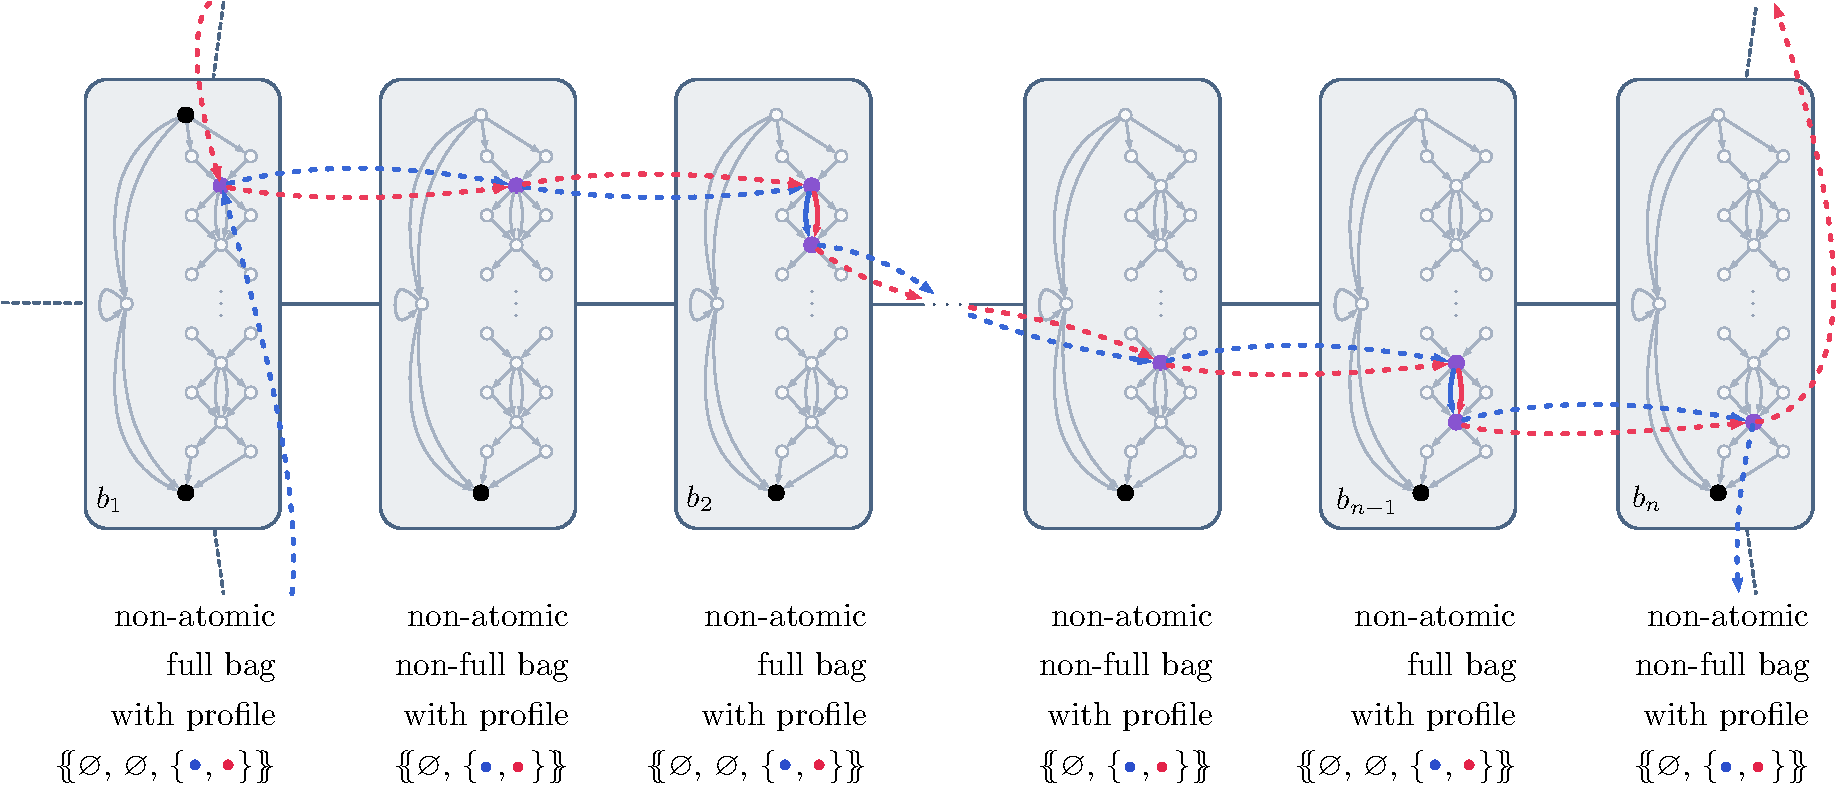
\includegraphics[width=\linewidth]{trio-tree-dec-long-path.pdf}
	\caption{
		\AP\label{fig:trio-tree-dec-long-path}
        "Profiles" of the "bags" in the "non-branching path" between $b_1$ and $b_n$ in the "fine tagged tree decomposition" obtained from \Cref{fig:trio-tree-dec} after applying 
		\Cref{lemma:locally_acyclic_treedec,fact:restriction_tagged_treedec} to both the
		red and blue "atom refinements".
	}
\end{figure*}

\begin{definition}[Types and Profiles]
    \AP Given a "trio" $\fun\colon \rho \surj \alpha$ and a "fine tagged tree decomposition"
    $(T, \bagmap, \tagmap)$ of $\fun$, for each "bag" $b$ of $T$, we say that:
    \begin{itemize}
        \itemAP $b$ is ``""atomic""'' if there is at least one atom $e \in \tagmap^{-1}[b]$ 
            and at least one variable $x$ of $e$ such that $x \in \vars{\gamma}$, "ie", the atom $e$ is not in the `middle' part of an "atom refinement";
        % \item $b$ is ``""atomic""'' if $b$ is "tagged" by an "atom" of $\gamma$, \ie~if
        %     $b = \tagmap(e)$ for some $e \in \atoms{\rho}$ where both endpoints of $e$ are variables of $\gamma$,
        %     \ie~were not created by "refinement";
        \itemAP otherwise, when $b$ is "non-atomic", we assign to each variable
            $z \in \bagmap(b) \subseteq \vertex{\alpha}$ a ""type@@stw""\phantomintro{\typeStw}
            \begin{align*}
                \reintro*\typeStw_z^b \defeq
                \bigl\{ x \atom{L} y \text{ "atom" of $\gamma$} \;\big\vert\; {} &
                    \text{the path "induced" by the "atom refinement"} \\
                    &\text{of $x \atom{L} y$ in $\rho$ "leaves" $b$ at $z$}
                \bigr\},
            \end{align*}
			where each "type@@stw" is potentially the empty set.
            Then the ""profile"" of $b$ is the multiset of the types of $z$
            when $z$ ranges over $\bagmap(b)$.
    \end{itemize}
\end{definition}

Note that $\rho$ and $\alpha$ can have arbitrarily more "atoms" than the original query
$\gamma$, and so the numbers of "bags" in $T$ can be arbitrarily high. However,
only few of them can be "atomic": an "atom refinement" of "atom" of $\gamma$
contains at most two "atoms" with a variable from $\gamma$---namely the
first and the last "atom" in the "refinement@atom refinement".
\begin{fact}
	\AP\label{fact:bound-atomic-bags}
	There is at most $2 \nbatoms{\gamma}$ "atomic bags" in $T$.
\end{fact}


Consider the "fine tree decomposition" of \Cref{fig:path-induced}, and now apply the construction of \Cref{lemma:locally_acyclic_treedec} to the red "atom refinement", followed by \Cref{fact:restriction_tagged_treedec}. We now obtain a "non-branching path"
between "bags" $b_1$ and $b_n$. We depict it in \Cref{fig:trio-tree-dec-long-path}:
the implicit "bags", hidden behind the dashed edges in \Cref{fig:path-induced} (see \Cref{nota:nice-tree-dec}), are made explicit in this new figure, and, moreover, the rest of the "fine tree decomposition" is not drawn.
Lastly, for each "bag", we indicate if it is "full" and if it is "atomic"; when it is not "atomic", 
we provide the "profile" of the "bag".

The rest of the proof consists in two parts.
First, we show that if two "non-atomic bags" $b$ and $b'$
occurring in some "non-branching path"
of $T$ have the same "profile", then we can essentially replace 
the path between $b$ and $b'$ by a path of constant length (\Cref{claim:shortening-paths}). And second, we show that in every sufficiently long "non-branching path"
we can find $b$ and $b'$ satisfying the aforementioned property: this
part simply relies on an enhanced ``pigeonhole principle'' (\Cref{fact:pigeon-hole}).

\begin{restatable}{clm}{shorteningpaths}
    \AP\label{claim:shortening-paths}
	Let $\fun\colon \rho \surj \alpha$ be a "trio", and consider a
	"fine tagged tree decomposition" of $f$ which is "locally acyclic".
    Suppose there are two "bags" $b$ and $b'$ such that:
	\begin{enumerate}
		\item they contain at most $k$ nodes ("ie", not "full" "bags"),
		\item they have the same "profile",
		\item there is a "non-branching path" in $T$ between these "bags", and
		\item no "bags" of the path between $b$ and $b'$ (both included) are "atomic".
	\end{enumerate}
	Then, there exists a "trio" $\fun'\colon \rho' \surj \alpha'$ and a
    "fine tagged tree decomposition" of $\fun'$ of "width" at most $k$
    that can be obtained by replacing the "non-branching path" between $b$ and $b'$
    in the "fine tagged tree decom\-position" of
    $\fun$ by another "non-branching path" with at most 
    $2k+1$ "bags", such that $\alpha \contained \alpha'$.
\end{restatable}
The proof of \Cref{claim:shortening-paths} relies on the definition of "profile", which
was specifically designed so that we can "condense" every "refinement" between $b$ and $b'$,
while preserving every needed property of the "trio".
We give first an informal and then a formal proof of \Cref{claim:shortening-paths}, which are 
illustrated in \Cref{fig:shortening-paths}.

\begin{figure*}
    \centering%
    \subfloat[An "approximation" $\alpha$.]{%
        \AP\label{fig:shortening-paths-approx}%
        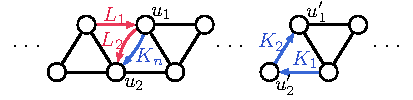
\includegraphics[width=.45\linewidth]{shortening-paths-approx.pdf}
    }
	\hfill
	\addtocounter{subfigure}{1}
    \subfloat[The resulting "approximation" $\alpha'$.]{%
        \AP\label{fig:shortening-paths-approx-result}%
        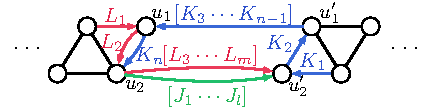
\includegraphics[width=.45\linewidth]{shortening-paths-approx-result.pdf}
    }\\[1em]
	\addtocounter{subfigure}{-2}
    \subfloat[A "fine tagged tree decomposition" of $\fun\colon \rho \surj \alpha$
    together with the "path induced" by three "atom refinements"
    of $\rho$ (in red, green \& blue).]{%
        \AP\label{fig:shortening-paths-tree-dec}%
        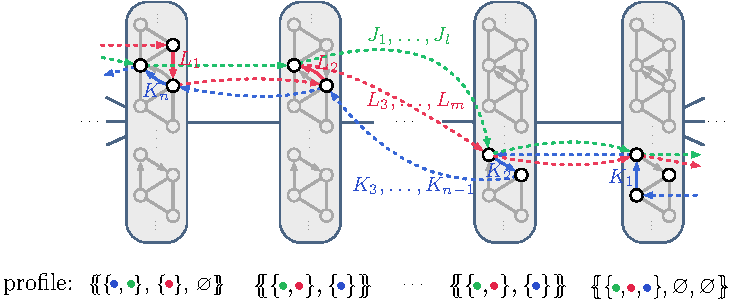
\includegraphics{shortening-paths-tree-dec.pdf}
    }
    \caption{%
        \AP\label{fig:shortening-paths}%
		A "trio" $\fun\colon \rho \surj \alpha$---where $\rho$ and $\fun$ are implicit---
		together with one of its "fine tagged tree decomposition"
		(\Cref{fig:shortening-paths-approx,fig:shortening-paths-tree-dec}).
		There are two non-"full bags" in the path with the same "profile", and thus the query $\alpha$ can be simplified to $\alpha'$
		(see \Cref{fig:shortening-paths-approx-result})
		by applying "condensations" to the "atom refinements" involved.
    }
\end{figure*}

\begin{proof}[Informal proof of \Cref{claim:shortening-paths}]
    \AP\label{proof-claim:shortening-paths}
    If $b$ and $b'$ have the same "profile", then in particular they have the same cardinality $m$,
    which is smaller or equal to $k$ by assumption.
    Let $\bagmap(b) = \{x_1,\dotsc, x_m\}$ and $\bagmap(b') = \{y_1,\dotsc,y_m\}$ be such that: 
    $\typeStw^{b}_{x_i} = \typeStw^{b'}_{y_i}$ for all $1 \leq i \leq m$.
	Note that the $x_i$'s don't need to be distinct from the $y_i$'s.
	Essentially, we can then "condense"
    every "atom refinement" in $\rho$ of some "atom" occurring in a set
    of the form $\typeStw^{b}_{x_i} = \typeStw^{b'}_{y_i}$ for some $i$.
	At this point, bags strictly comprised between
    $b$ and $b'$ are discarded, and so are variables of $\alpha$ that do not occur anywhere else.
    We are left with two halves of a "fine tagged tree decomposition" that we need to merge,
    which can easily be done by using \Cref{prop:connecting-tree-decompositions}.
    The construction makes use of some crucial ingredients to guarantee its correctness.
    \begin{itemize}
        \item First, an "atom" $y \atom{L} y'$ of $\gamma$ cannot occur
            in two different "types@@stw", allowing us to do the "condensation" of each "atom refinement" independently---this property is guaranteed by the fact that we started
			with a "locally acyclic" "fine tagged tree decomposition", so an "atom" of $\gamma$ cannot leave a given "bag" at two different variables, by
			\Cref{fact:acyclic-decomposition-leave-forever}.
        \item Second, this "condensation" forces us to add new "atoms" in $\alpha$ (to preserve the
            existence of a "homomorphism" from the "refinement" to the approximation)
            from some variables of $\bagmap(b)$ to some variables of $\bagmap(b')$,
            but we only add edges from $x_i$ to $y_i$, and never from $x_i$ to $y_j$ with
			$i \neq j$. This allows us to preserve the "tree-width" of the approximation
			by using \Cref{prop:connecting-tree-decompositions}.\qedhere
    \end{itemize}
\end{proof}

\begin{proof}[Formal proof of \Cref{claim:shortening-paths}]
    Let
    \[\bagmap(b) = \{x_1,\dotsc, x_m\}
    \text{ and }
    \bagmap(b') =\{y_1,\dotsc,y_m\}
    \]
    be as in the informal proof.
    Note that given an "atom" $x \atom{L} y$ of $\gamma$ and
	a "bag", there is at most
    one variable of $\alpha$ "st" $x \atom{L} y$ is in the "type@@stw" of this variable
	at this bag, by \Cref{fact:acyclic-decomposition-leave-forever}.
	% Symbolically: for all $b \in T$, for all $x, y \in \bagmap(b)$,
	% if $\typeStw_x^b = \typeStw_y^b$, then $x=y$.

    For every "atom" $x \atom{L} y$ of $\gamma$, let 
    $\pi(x \atom{L} y) \defeq t_0 \atom{L_1} \dotsc \atom{L_n} t_n$
    be its "refinement" in $\rho$.
    If $x \atom{L} y$ is not in some "type@@stw" of the "profile" of $b$
    (or equivalently, of $b'$), leave it as is.
    Otherwise, let $i$ (resp.\ $j$) be the unique
    index (by acyclicity) such that
    $\tagmappath{t_0 \atom{L_1} \dotsc \atom{L_n} t_n}$ "leaves" $b$
    at $\fun(t_i)$ (resp.\ "leaves" $b'$ at $\fun(t_j)$).
    Define
    \[
		\pi'(x \atom{L} y) \defeq
        t_0 \atom{L_1} \dotsc \atom{L_i} t_i \atom{\contract{L_{i+1}\cdots L_j}}
        t_j \atom{L_{j+1}} \dotsc \atom{L_n} t_n
    \]
    when $i \leq j$ and otherwise the definition is symmetric.
    Then, let $\rho'$ be the "refinement" of $\gamma$ obtained by simultaneously
    substituting $\pi(x \atom{L} y)$ with $\pi'(x\atom{L} y)$  in $\rho$,
    for every "atom" $x\atom{L} y$ of $\gamma$.

    Then, let $\alpha'$ be the query obtained by first
    adding the atoms  
    \[\fun(t_i) \atom{\contract{L_{i+1}\cdots L_j}} \fun(t_j),\]
    and observe that $\fun\colon \rho \surj \alpha$
    induces a "homomorphism" $\fun'\colon \rho' \homto \alpha'$---in particular, note that
	because of assumption (4) of our claim, we could not have removed images of
	free variables of $\gamma$.
    Moreover, by construction, $\alpha \contained \alpha'$ (by \Cref{fact:refinement-contained}).
	As usual, we restrict $\alpha'$ to the image of $f'$ so that it
	becomes "strong onto", while preserving that fact that $\alpha \contained \alpha'$.
	Finally, we build a "tagged tree decomposition" $(T', \bagmap', \tagmap')$
    of $f'$ by applying \Cref{prop:connecting-tree-decompositions}; it can be applied because:
	\begin{itemize}
		\item by assumption $(1)$ and $(2)$ of the claim, both "bags" have the same cardinality $m \leq k$;
		\item the variables in common between the first and second half of the "decomposition@fine tagged tree decomposition" are necessarily included in $Z \defeq \bagmap(b) \cap \bagmap(b')$
		since we started from a "tree decomposition";
		\item we only add atoms from $x_i$ to $y_i$: depending on whether $x_i \in^? Z$,
		and whether $y_i \in^? Z$, we fall in one of the four types of atoms allowed
		by \Cref{prop:connecting-tree-decompositions}.
	\end{itemize}
	This concludes the proof of \Cref{claim:shortening-paths}.
\end{proof}

\begin{figure}[tbp]
	\centering
    \subfloat["Non-branching path" in the ``new'' "fine tagged tree decomposition".]{%
        \AP\label{fig:trio-tree-dec-long-path-shortened}%
        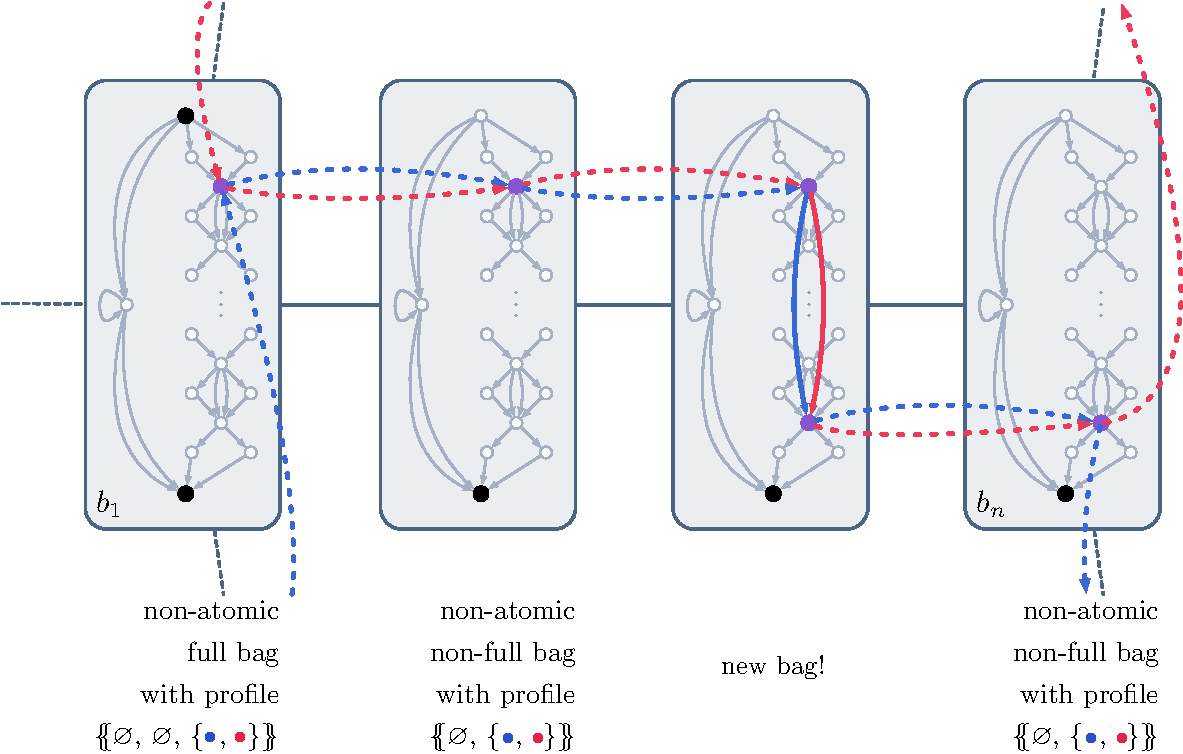
\includegraphics[width=\linewidth]{trio-tree-dec-long-path-shortened.pdf}
    }\\[1em]
    \subfloat[The original query $\gamma$ of "tree-width" 3.]{%
        \AP\label{fig:trio-result-query}%
        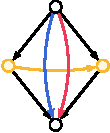
\includegraphics[width=.2\linewidth]{trio-query.pdf}
    }
	\hfill
    \subfloat[The ``new'' "refinement" $\rho'$ of $\gamma$.]{%
        \AP\label{fig:trio-result-refinement}
        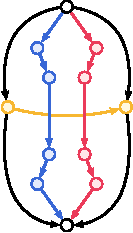
\includegraphics[width=.28\linewidth]{trio-refinement-result.pdf}
    }
	\hfill
    \subfloat[The ``new'' "approximation" $\alpha'$ of "tree-width" 2.]{
        \AP\label{fig:trio-result-approx}
        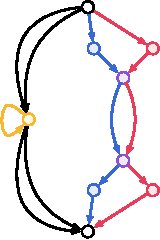
\includegraphics[width=.3\linewidth]{trio-approximation-result.pdf}
    }
	\caption{
		\AP\label{fig:trio-result}
		"Trio" resulting from applying \Cref{claim:shortening-paths}
		between the second and last "bags" of \Cref{fig:trio-tree-dec-long-path}.
	}
\end{figure}
In \Cref{fig:trio-tree-dec-long-path-shortened}, we depict the "non-branching path" (the rest
of the "fine tree decomposition" is not depicted as it is left unchanged) obtained
by applying the construction used to prove \Cref{claim:shortening-paths}
between the second and last bag of \Cref{fig:trio-tree-dec-long-path}. Observe that a "non-branching path" of size $\+O(n)$ is replaced, by this procedure, by a path with three "bags".
Then, after applying \Cref{fact:restriction_tagged_treedec}, we obtain a "trio"
depicted in \Cref{fig:trio-result-query,fig:trio-result-refinement,fig:trio-result-approx}.

Before moving to the proof of \Cref{lemma:shape-decomposition}, we establish one last result.
\begin{fact}
    \AP\label{fact:pigeon-hole}
    Let $n, d, t \in \N$. Let $P$ be a set with at most $n$ elements,
    and $\tilde P$ be the disjoint union of $P$ and $\{\trap, \avoid\}$.
    For every natural number $m \geq 2(t+1)d(n+1) + 2t$, 
    for every sequence $(p_i)_{0 \leq i < m} \in \tilde P^m$ containing at most
    $t$ elements equal to $\trap$, if at most half of  the elements of the sequence
    are equal to $\avoid$, then there exists
    $i < i'$ such that $p_i = p_{i'} \neq \avoid$, $i' - i \geq d$ and
    $p_j \neq \trap$ for every $i \leq j \leq i'$.
\end{fact}

\begin{proof}
    First extract from $(x_i)_{0 \leq i < m}$ the subsequence of elements
    distinct from $\avoid$, of length at least $\lceil\frac{m}{2}\rceil \geq (t+1)d(n+1) + t$.
    Then extract from it contiguous subsequences that avoid
    the $\trap$ element. Since there is at most $t+1$ subsequences like this,
    one of them must have size at least $d(n+1)$. Denote by
    $(y_i)_{0 \leq i < d(n+1)}$ the prefix of such a subsequence.
    Applying the pigeon-hole principle
    to $(y_{i\cdot d})_{0 \leq i < n+1}$ yields the desired result.
\end{proof}

\begin{proof}[Proof of \Cref{lemma:shape-decomposition}]
    Let $\fun\colon \rho \surj \alpha$ be a "trio", and $(T, \bagmap, \tagmap)$ be a
    "locally acyclic" "fine tagged tree decomposition" of $\fun$. If there is a "non-branching path"
    $(b_i)_{0\leq i<m}$ in $T$ of length at least $m$, let $(p_i)_{0 \leq i<m}$ be
    the sequence defined by letting:
    \[
        p_i \defeq \begin{cases}
            \trap & \text{if $b_i$ is "atomic",} \\
            \avoid & \text{if $b_i$ contains $k+1$ variables,} \\
            \text{"profile" of } b_i & \text{otherwise.}
        \end{cases}    
    \]
    
    Observe that, by \Cref{fact:acyclic-decomposition-leave-forever},
	"profiles" can be seen encoded as partial functions from the set of "atoms" of $\gamma$ to $\lBrack 1,k\rBrack$---of course this encoding is not surjective---, so
	there are at most $(k+1)^{\nbatoms{\gamma}}$ different "profiles" on "bags" with at most $k$ variables.
    Applying \Cref{fact:pigeon-hole} for $n = (k+1)^{\nbatoms{\gamma}}$, $d = 2k+1$, $t = 2\nbatoms{\gamma}$ yields, under the assumption that
    \[
        m \geq m_0 \defeq 2(2\nbatoms{\gamma}+1)(2k+1)((k+1)^{\nbatoms{\gamma}}+1)
		+ 4\nbatoms{\gamma},
    \]
    the existence of indices $i < i'$ such that $i' - i \geq 2k+1$,
    and $b_i$ and $b_{i'}$ have the same "profile", contain at most $k$ variables,
    and every bag $b_j$ for $i \leq j \leq i'$ is "non-atomic"---note that the hypothesis
    of \Cref{fact:pigeon-hole} are satisfied since at most $t = 2\nbatoms{\gamma}$
    "bags" of $(b_i)_{0 \leq i < m}$ are "atomic" ("cf" \Cref{fact:bound-atomic-bags}), and assuming "wlog"~that
    no two consecutive "bags" of $(b_i)_{0 \leq i < m}$ are identical, since the "tagged tree decomposition" $(T, \bagmap, \tagmap)$ of "width" $k$ is "fine", at most half of the 
    "bags" contain $k+1$ variables.
    The assumption $i' - i \geq 2k+1$ means that the path from $b_i$ to $b_{i'}$ has
    length at least $2k+2$, and thus applying \Cref{claim:shortening-paths} will
    strictly shorten this path.
    Note that \Cref{claim:shortening-paths} preserves the "fineness" of the "tagged 
    tree decomposition", its "local acyclicity", and that the size of
    this "tree decomposition" is strictly smaller (in number of nodes) than
    the original "tree decomposition". By iteratively applying this construction,
    we obtain a "trio" $\fun'\colon \rho' \surj \alpha'$ together with a "locally acyclic"
    "fine tagged tree decomposition" $T'$
    of "width" at most $k$, such that $\alpha \contained \alpha'$ (by a variation of
	\Cref{fact:refinement-contained})
    and every "non-branching path" of $T'$ has length at most\footnote{Recall that $k$
	is fixed.} 
    $m_0 - 1 \in 
    \+O(\nbatoms{\gamma}\cdot (k+1)^{\nbatoms{\gamma}})$.
\end{proof}

\subsection{\AP{}Proof of Lemma~\ref{lemma:bound_size_refinements}}
\label{sec:proof-bound-size-refinements}

Finally, our main lemma follows from
\Cref{lemma:locally_acyclic_treedec,lemma:shape-decomposition}.

\begin{proof}[Proof of \Cref{lemma:bound_size_refinements}]
    In order to show $\MUA{\gamma}{\Tw} \contained \MUAHomBounded{\gamma}{\Tw}{\leq\l}$---the other
    "containment" being trivial---, pick a "trio" $\fun\colon \rho \surj \alpha$.
    Applying \Cref{lemma:locally_acyclic_treedec} and then \Cref{lemma:shape-decomposition}
    yields the existence of a "trio" $\fun'\colon \rho' \surj \alpha'$ together
    with a "fine tagged tree decomposition" $(T', \bagmap', \tagmap')$ of $\fun'$
    such that $\alpha \contained \alpha'$ and $(T', \bagmap', \tagmap')$ is "locally acyclic",
    and any "non-branching path" in $T'$ has length at most
    $\+O(\nbatoms{\gamma}\cdot (k+1)^{\nbatoms{\gamma}})$.

    Moreover, we can assume "wlog", by applying \Cref{fact:restriction_tagged_treedec},
    that every leaf of $T'$ is "tagged" by at least one "atom" of $\rho'$.
    The "local acyclicity" of $T'$ implies that if $b$ is a leaf of $T'$,
    and
    $
        \pi \defeq x \atom{L_1} t_1 \atom{L_2} \cdots \atom{L_{n-1}} t_{n-1} \atom{L_n} y
    $
    is an "atom refinement" in $\rho'$ of some "atom" $x \atom{L} y$ of $\gamma$,
    then if $b$ is tagged by one "atom" of $\pi$ this "atom" must either be $z_0 \atom{L_1} z_1$
    or $z_{n-1} \atom{L_n} z_n$ by "local acyclicity".
    The number of such "atoms" in $\rho'$ being bounded by $2\nbatoms{\gamma}$, we conclude that
    $T'$ has at most $2\nbatoms{\gamma}$ leaves.

    Then, observe that a tree with at most $p$ leaves and whose "non-branching paths"
    have length at most $q$ is of height at most\footnote{The length of a path being its number of nodes,
    and with the convention that the height of a single node is zero.} $p\cdot q - 1$. We
    conclude that the height of $T'$ is 
    $\+O(\nbatoms[2]{\gamma}\cdot (k+1)^{\nbatoms{\gamma}})$.
    Using again the "local acyclicity" of $T'$, observe that the "refinement length" of $\rho'$
    is at most twice the height of $T'$, and hence $\rho' \in \Refin[\leq \l](\gamma)$
    where $\l = \Theta(\nbatoms[2]{\gamma}\cdot (k+1)^{\nbatoms{\gamma}})$.
    In other words, $\alpha' \in \MUAHomBounded{\gamma}{\Tw}{\leq\l}$.
    Hence, we have shown that for all $\alpha \in \MUAHom{\gamma}{\Tw}$,
    there exists $\alpha' \in \MUAHomBounded{\gamma}{\Tw}{\leq\l}$ such that $\alpha \contained \alpha'$.
\end{proof}

This concludes \Cref{sec:proof-key-lemma} and the proof of the "Key Lemma".
The next four sections are independent of one another:
\begin{itemize}
	\item in \Cref{sec:sre}, we show that the "2ExpSpace" complexity
	of the "semantic tree-width $k$ problem" can be dropped down to
	"PiP2" under assumptions on the regular languages;
	\item in \Cref{sec:acyclic-queries,sec:semantic-path-width}, we adapt
	the proofs of this section to deal with
	"semantic tree-width" 1 and "semantic path-width" $k$, respectively.
	\item in \Cref{sec:lowerbound}, we prove an "ExpSpace" lower bound for the
	"semantic tree-width $k$ problem" and "semantic path-width $k$ problems";
\end{itemize}

